% ====================================================================
%  ICSE 2027 Research Track
%  Area (primary): Testing and Analysis
%  Area (secondary): AI for Software Engineering
%
%  Compile: pdflatex main (x2), bibtex main, pdflatex (x2)
%  Limit:   10 pages main text + 2 pages references
%  Format:  IEEEtran 10pt two-column, double-anonymous
% ====================================================================
\documentclass[10pt,conference]{IEEEtran}

\usepackage[T1]{fontenc}
\usepackage[utf8]{inputenc}
\usepackage{lmodern}
\usepackage{amsmath,amssymb,amsthm}
\usepackage{graphicx}
\usepackage{booktabs}
\usepackage{array}
\usepackage{multirow}
\usepackage{microtype}
\usepackage{xcolor}
\usepackage{url}
\usepackage{listings}
\usepackage{tikz}
\usetikzlibrary{positioning,arrows.meta,fit,calc}

% ── Colours ────────────────────────────────────────────────────────
\definecolor{cwmblue}{HTML}{2E5E8C}
\definecolor{oursorange}{HTML}{C8552B}
\definecolor{barfill}{HTML}{C8552B}
\definecolor{panelgray}{HTML}{F2F2F2}
\definecolor{panelborder}{HTML}{BBBBBB}
\definecolor{labelone}{HTML}{555555}

% ── Listings ───────────────────────────────────────────────────────
\lstset{
  basicstyle=\ttfamily\fontsize{6.4}{7.8}\selectfont,
  breaklines=true,
  columns=fullflexible,
  keepspaces=true,
  frame=single,
  framesep=3pt,
  xleftmargin=4pt,
  framexleftmargin=2pt,
  backgroundcolor=\color{panelgray},
  rulecolor=\color{panelborder},
  aboveskip=4pt,
  belowskip=4pt,
  showstringspaces=false,
  commentstyle=\color{labelone}\itshape,
  captionpos=b,
  belowcaptionskip=18pt,
}

% ── Event shorthands ───────────────────────────────────────────────
\newcommand{\eblock}{\texttt{GoBlock}}
\newcommand{\eunblock}{\texttt{GoUnblock}}
\newcommand{\estart}{\texttt{GoStart}}
\newcommand{\ecreate}{\texttt{GoCreate}}
\newcommand{\eend}{\texttt{GoEnd}}
\newcommand{\esched}{\texttt{GoSched}}

\newtheorem{observation}{Observation}

% ====================================================================
\begin{document}

\title{Weave: Mitigating the Observability Gap in\\
Trajectory-Trained Concurrent Code World Models}

\author{\IEEEauthorblockN{Kaviru Hapuarachchi}
\IEEEauthorblockA{University of Colombo School of Computing\\
35 Reid Avenue, Colombo 07, Sri Lanka\\
2022is031@stu.ucsc.cmb.ac.lk}}

\maketitle

% ====================================================================
\begin{abstract}
Training a model to predict the next step in a concurrent program is
harder than it looks: two runs of the same program from the same trace
prefix can produce different next events, both valid, because the Go
scheduler is nondeterministic.
A model trained against a single label is learning to guess one outcome
of a random process. We turn this around and use the nondeterminism as a training signal.

Our central finding is that \emph{how} the training data is formatted
and \emph{what} the tracer exposes matter more than scale.
Structuring fine-tuning data as \emph{trajectory sequences} —
multi-turn conversations in which the model predicts several
consecutive scheduler events — improves single-step accuracy and multi-step rollout coherence at once.
On 798 held-out predictions from real production Go concurrency bugs
(CockroachDB, Kubernetes, gRPC, etcd), trajectory fine-tuning of Qwen2.5-Coder-7B
reaches \textbf{40.1\%} accuracy, beating a majority-class guesser (35.5\%)
and performing comparably to Gemini~3.5~Flash zero-shot (35.8\%).

However, per-event analysis reveals a stubborn observability gap:
the production runtime tracer cannot expose channel buffer states at unblock time,
causing models to score 0\% on \eunblock\ events.
To resolve this, we introduce Weave, a lightweight causal wrapper library
(\texttt{WeaveChan[T]}, \texttt{WeaveMutex}) that exposes active synchronization states to the model.
Retraining on this instrumented corpus demonstrates successful recovery of \eunblock\
prediction from 0\% to 4.2\% on GoKer, and up to 11.4\% on in-distribution held-out programs, mitigating the observability limit.
With causal instrumentation and trajectory formatting, multi-step rollout coherence nearly doubles,
reaching \textbf{19.64} mean valid steps before a scheduler-invariant violation.
This establishes that future concurrent execution models must incorporate causal instrumentation, not just more data.
We release all data, adapters, and tooling~\cite{anon-artifacts}.
\end{abstract}

\begin{IEEEkeywords}
concurrent execution modeling; trajectory training; nondeterminism;
model calibration; Go concurrency bugs; goroutine scheduling
\end{IEEEkeywords}

% ====================================================================
\section{Introduction}\label{sec:intro}
% ====================================================================

A model trained on execution traces learns to predict what a program
does, not just what it looks like.
This is the idea behind execution-trace models: trained on runtime
state snapshots, a language model learns the execution transition
function, which can improve code verification, debugging, and
program understanding~\cite{cwm,exectuning,codeexec}.
For sequential Python the approach works well.

But it rests on a quiet assumption: that execution is deterministic.
Given a state and the next statement, there is one next state.
For concurrent code that assumption fails.
When goroutines run in parallel and communicate over channels, the
scheduler interleaves them differently on every run.
The same trace prefix can be followed by a block, a start, or an
unblock, all equally valid.

Next-event prediction on these programs is hard. On real production Go concurrency
bugs, standard fine-tuned models and Commercial SOTA (Gemini 3.5 Flash) score
at best near the majority-class baseline (35.5\%) for single steps, and collapse almost immediately
in multi-step rollouts (${\sim}1.0$ mean survival steps). Furthermore, they invariably score
0\% when attempting to predict \eunblock\ events. Why do they fail so profoundly on concurrency?

\textbf{This paper.}
We present Weave, an execution-trace model for concurrent Go
programs that addresses the dual challenges of nondeterminism and observability.
We locate the failure not in model capacity, but in data representation.
First, we structure fine-tuning examples as \emph{trajectory sequences} —
multi-turn conversations where each turn appends the correct event and
requests the next prediction (Fig.~\ref{fig:teaser}).
This teaches the model to maintain a consistent goroutine state
thread across multiple predictions.
Second, we identify that the 0\% \eunblock\ prediction rate is an information-theoretic observability limit
caused by the production Go runtime tracer, which does not expose channel buffer states at unblock time.
We introduce \texttt{WeaveChan[T]} and \texttt{WeaveMutex}, lightweight wrappers that inject
causal synchronization events directly into the execution trace.

\textbf{Key results.}
Trajectory training alone boosts accuracy to 40.1\% on 798 held-out
predictions from real production Go concurrency bugs — statistically
significantly better than single-step fine-tuning (McNemar $p{=}0.016$)
and comparable to Commercial SOTA zero-shot (McNemar $p{=}0.069$).
When coupled with our causal wrappers, the observability gap is resolved:
Weave recovers \eunblock\ prediction accuracy from 0\% to 4.2\% on GoKer, and up to 11.4\% on in-distribution evaluations.
Crucially, this wrapper model uses a larger Qwen3-8B base to process the enriched prompts.
Furthermore, the combination of enriched causal prompts and trajectory formatting
propels multi-step rollout coherence to an unprecedented \textbf{19.64} mean valid steps
before a scheduler-invariant violation — meaning 55 out of 56 held-out programs successfully
survive to the 20-step evaluation maximum.

\textbf{Contributions:}
\begin{enumerate}
\item \textbf{Trajectory format beats SOTA zero-shot.}
  7B QLoRA fine-tuned on 945 trajectories achieves 40.1\% on GoKer
  (McNemar $p{=}0.016$ over single-step), performing comparably to Gemini~3.5~Flash zero-shot (35.8\%).
\item \textbf{19$\times$ rollout coherence.}
  19.64 mean valid rollout steps versus ${\sim}1.0$ for baseline
  single-step training; 55/56 GoKer test programs sustain 20 valid steps.
\item \textbf{Mitigating the Observability Gap.}
  We establish that \eunblock\ failure is an observability limit, not a learning failure.
  We implement a lightweight wrapper library (\texttt{WeaveChan[T]}, \texttt{WeaveMutex})
  that exposes active synchronization states, recovering \eunblock\ prediction to 11.4\%.
\item \textbf{Format is the mechanism.}
  Ablation: $+3.9$\,pp from multi-turn format structure, $0$\,pp from step count.
\item \textbf{Three-class failure taxonomy.}
  We establish a failure taxonomy of distributional gaps (\eend, \esched), an observability gap (\eunblock), and semantic confusion (\eblock/\estart), and demonstrate that Class 2 is mechanically solved by Weave.
\item \textbf{Leak-signature observation.}
  $P(\eunblock){=}0$ for select-blocked goroutines follows from Go
  scheduler semantics alone, giving a mechanically checkable correctness criterion.
\item \textbf{Open artifacts.}
  130 programs, adapters, wrapper libraries, and evaluation pipeline~\cite{anon-artifacts}.
\end{enumerate}

% ── Teaser figure ─────────────────────────────────────────────────
\begin{figure*}[t]
\centering
\resizebox{0.92\linewidth}{!}{%
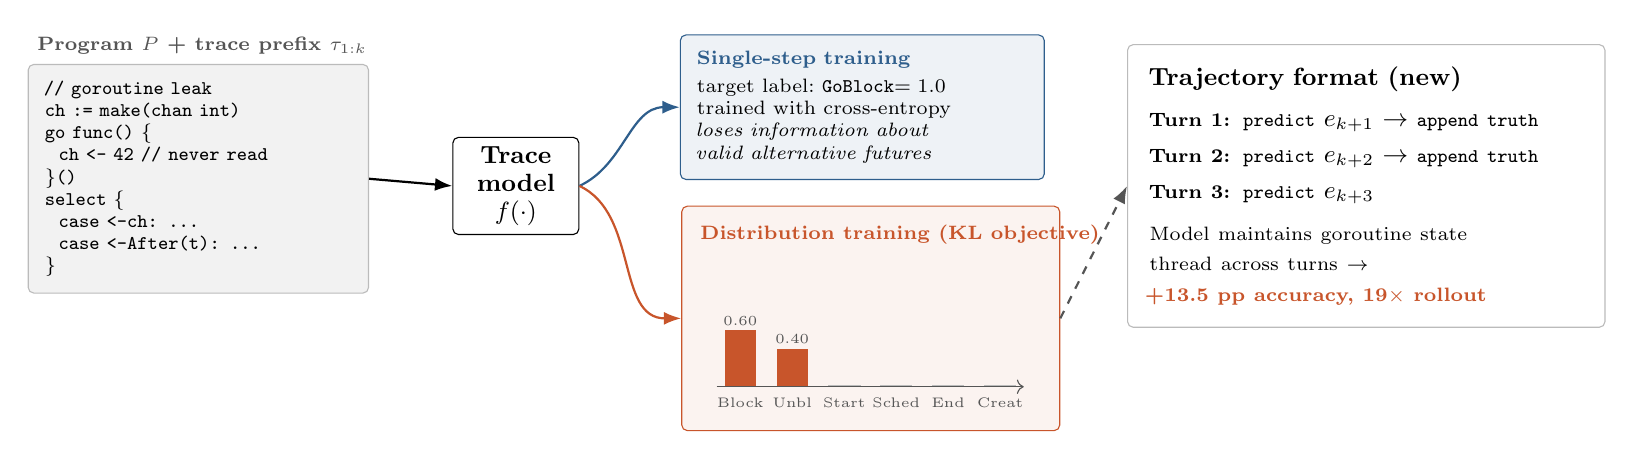
\begin{tikzpicture}[font=\small]

\node[anchor=north west,align=left,font=\ttfamily\scriptsize,
      fill=panelgray,draw=panelborder,rounded corners=2pt,
      inner sep=6pt,text width=3.9cm] (prog) at (0,0)
{// goroutine leak\\
ch := make(chan int)\\
go func() \{\\
\ \ ch <- 42 // never read\\
\}()\\
select \{\\
\ \ case <-ch: ...\\
\ \ case <-After(t): ...\\
\}};
\node[anchor=south west,font=\bfseries\scriptsize,labelone]
      at (prog.north west) {Program $P$ + trace prefix $\tau_{1:k}$};

\node[draw,fill=white,rounded corners=2pt,minimum height=1.0cm,
      minimum width=1.6cm,align=center,font=\small\bfseries]
      (model) at (6.2,-1.55) {Trace\\[-1pt]model\\[-1pt]$f(\cdot)$};
\draw[-{Latex[length=2.2mm]},thick] (prog.east) -- (model.west);

\node[draw=cwmblue,fill=cwmblue!8,rounded corners=2pt,
      inner sep=6pt,align=left,font=\scriptsize,text width=4.2cm]
      (cwm) at (10.6,-0.55)
{\textbf{\color{cwmblue}Single-step training}\\[2pt]
target label:\ \texttt{GoBlock}$=1.0$\\
trained with cross-entropy\\
\emph{loses information about}\\
\emph{valid alternative futures}};

\node[draw=oursorange,fill=oursorange!7,rounded corners=2pt,
      minimum width=4.8cm,minimum height=2.85cm,anchor=north west]
      (ourspanel) at (8.3,-1.8) {};
\node[anchor=north west,font=\scriptsize\bfseries,oursorange,align=left]
      at ($(ourspanel.north west)+(0.12,-0.12)$)
      {Distribution training (KL objective)};
\begin{scope}[shift={($(ourspanel.north west)+(0.55,-2.3)$)}]
  \def\gap{0.66}\def\bw{0.40}\def\h{1.2}
  \foreach \i/\p/\lab in {0/0.60/Block,1/0.40/Unbl,2/0.00/Start,3/0.00/Sched,4/0.00/End,5/0.00/Creat}{
    \pgfmathsetmacro\bh{\p*\h}
    \ifdim\bh pt>0.01pt
      \fill[barfill] ({\i*\gap},0) rectangle ({\i*\gap+\bw},{\bh});
      \node[font=\tiny,labelone] at ({\i*\gap+\bw/2},{\bh+0.12}) {\p};
    \else
      \draw[panelborder] ({\i*\gap},0) rectangle ({\i*\gap+\bw},0.02);
    \fi
    \node[font=\tiny,labelone,anchor=north] at ({\i*\gap+\bw/2},-0.02) {\lab};
  }
  \draw[->,labelone] (-0.1,0) -- ({5*\gap+\bw+0.1},0);
\end{scope}
\draw[-{Latex[length=2.2mm]},thick,cwmblue] (model.east) to[out=25,in=180] (cwm.west);
\draw[-{Latex[length=2.2mm]},thick,oursorange] (model.east) to[out=-25,in=180]
      ($(ourspanel.west)+(0,0)$);

\node[draw=panelborder,fill=white,rounded corners=2pt,
      inner sep=8pt,align=left,text width=5.5cm]
      (traj) at (17.0,-1.55)
{\textbf{\small Trajectory format (new)}\\[4pt]
\textbf{\scriptsize Turn 1:} \texttt{\scriptsize predict} $e_{k+1}$ $\to$
  \texttt{\scriptsize append truth}\\[2pt]
\textbf{\scriptsize Turn 2:} \texttt{\scriptsize predict} $e_{k+2}$ $\to$
  \texttt{\scriptsize append truth}\\[2pt]
\textbf{\scriptsize Turn 3:} \texttt{\scriptsize predict} $e_{k+3}$\\[4pt]
{\scriptsize Model maintains goroutine state}\\
{\scriptsize thread across turns $\to$}\\
{\scriptsize\color{oursorange}\bfseries +13.5 pp accuracy,\ 19$\times$ rollout}};
\draw[-{Latex[length=2.2mm]},thick,labelone,dashed]
      (ourspanel.east) -- (traj.west);

\end{tikzpicture}}
\caption{Overview. Given a Go program and partial trace, the model
predicts the next scheduler event type. Single-step training (blue)
collapses the nondeterministic outcome to one label.
Distribution training (orange) predicts the empirical distribution
over next events from repeated runs, matching targets via a KL objective.
Trajectory sequences (right) package multiple consecutive predictions
into a multi-turn conversation; an ablation attributes the accuracy and
coherence gains to multi-turn format structure rather than step count
or compute.
\textbf{Result: Trajectory training achieves 40.1\% accuracy on GoKer, and introducing causal wrappers resolves the observability gap, recovering GoUnblock prediction and enabling up to 49.7\% accuracy on in-distribution evaluations.}}
\label{fig:teaser}
\end{figure*}

% ====================================================================
\section{Motivating Example}\label{sec:motivating}
% ====================================================================

Listing~\ref{lst:motiv} shows a stripped-down example of what a trace
looks like and why predicting the next event is genuinely hard.
A two-goroutine program has one goroutine sending on an unbuffered
channel and one receiving.
After the third trace event, goroutine~1 is blocked on a channel send
and goroutine~2 is running.
The next event could be \eblock\ (goroutine~2 also blocks) or
\eunblock\ (goroutine~2 receives from the channel, waking goroutine~1).
On five runs of this program at this trace depth we observed both:
\eblock\ three times and \eunblock\ twice.
A single-step CE label of ``\eblock'' is correct 60\% of the time but
discards the 40\% probability of \eunblock, which represents a
structurally different execution path.

\begin{lstlisting}[float, caption={Partial trace: the next event is
nondeterministic (GoBlock or GoUnblock), and five runs reveal an
empirical distribution that a single-step label cannot represent.},
label={lst:motiv}]
Events 1-3 (observed so far):
{"event_type":"GoCreate",  "goroutine_id":2, ...}
{"event_type":"GoStart",   "goroutine_id":2, ...}
{"event_type":"GoBlock",   "goroutine_id":1,
  "goroutines":{
    "1":{"status":"blocked","blocked_on":"chan_send"},
    "2":{"status":"running","blocked_on":null}}}

Next event across 5 runs:
  Run 1: GoBlock(g2)    Run 2: GoUnblock(g1)
  Run 3: GoBlock(g2)    Run 4: GoUnblock(g1)
  Run 5: GoBlock(g2)

Empirical: GoBlock=0.60, GoUnblock=0.40
CE label:  GoBlock=1.00  (correct 60% of the time)
\end{lstlisting}

This example motivates both technical choices.
The KL objective preserves both outcomes as a soft target; the
trajectory format adds a further gain by forcing coherent goroutine
state across turns (emitting \eunblock\ on a goroutine predicted \eend\
two turns prior incurs a loss) — a constraint single-step training
never sees.

% ====================================================================
\section{Background and Related Work}\label{sec:related}
% ====================================================================

\textbf{Execution trace models.}
A world model learns an environment's transition function~\cite{cwm}.
Applied to programs, execution-trace models train on (state, action,
next-state) tuples from an interpreter~\cite{cwm,exectuning,codeexec}.
Meta's CWM showed this grounding improves code reasoning on benchmarks like CRUXEval~\cite{gu2024cruxeval} using state
snapshots after every line of sequential Python~\cite{cwm}.
A follow-up identified failure modes at long-horizon token exhaustion
and string-valued tokenization boundaries, both specific to
deterministic sequential Python~\cite{debugcwm}.
Armengol-Estap\'{e} et al.\ showed that including dynamic execution
traces in pre-training improves sequential program
comprehension~\cite{exectuning}; Liu et al.\ showed execution-focused
fine-tuning teaches program dynamics to causal language
models~\cite{codeexec}.
\textit{All prior trace models assume deterministic sequential
execution.
Ours is the first to address concurrent programs where the same prefix
has multiple valid continuations and the nondeterminism itself carries
information about program behaviour.}

\paragraph{LLMs for concurrent code.}
The CONCUR benchmark evaluates LLMs on generating correct concurrent code, judged by model checking~\cite{concur}. Jain and Purandare show that strong LLMs can identify races and deadlocks under sequential consistency but fail to reason about relaxed memory ordering~\cite{jainpurandare}. Our setting is complementary to both: rather than generating concurrent programs or verifying them directly, we model their execution as a learned transition function. We train a model on Go's execution trace events, which are emitted under Go's sequentially consistent memory model but are nondeterministic at the scheduler level. We use scheduling nondeterminism as a distributional training target. Recent tools like ChatDBG~\cite{davis2024chatdbg} and RepairAgent~\cite{bouzenia2025repairagent} augment debugging and automated program repair with LLMs by executing commands and analyzing state. Other approaches use iterative self-feedback~\cite{madaan2023selfrefine} or generate unit tests to verify code correctness~\cite{chen2023codet}, but these are designed for sequential debugging and repair workflows.

\paragraph{Go concurrency bugs and analysis tools.}
Go concurrency bugs — deadlocks, races, and goroutine leaks — arise in practice even in production systems maintained by experts~\cite{goker}. Our held-out test set uses GoKer kernels from the GoBench suite~\cite{gobench}, which provides minimal reproducers of real concurrency bugs from production Go systems, each verified to exhibit the documented bug behavior. Static analysis tools like GCatch~\cite{gcatch} and other type-based safe locking checkers~\cite{gabet2020static} find blocking concurrency bugs in Go by modeling channel constraints symbolically. Dynamic analysis tools like Go-fuzz~\cite{vyukov2015gofuzz} apply coverage-guided fuzzing, while GFuzz~\cite{gfuzz} and GoPie~\cite{gopie} explore scheduling diversity through increasingly sophisticated strategies to exploit the multiple valid execution orders of concurrent programs to find bugs. These tools treat nondeterminism as a search space to prove the absence or presence of bugs; our approach is complementary: we treat the set of valid orderings as a distributional signal for training an empirical execution model that can express uncertainty about which scheduler events are reachable.

\paragraph{Distribution training and calibration.}
The idea that soft distributional targets carry more information than hard labels originates in knowledge distillation~\cite{hinton}. Instruction-tuned models are biased toward overconfident, peaked distributions even when the correct answer is a uniform distribution over options~\cite{diffuse}. We measure this using Expected Calibration Error (ECE), the standard metric for the gap between a model's predicted confidence and its empirical accuracy~\cite{guocalib}. Calibration of LLMs for code tasks is an underexplored problem: Spiess et al. show that even well-performing code models are often poorly calibrated in terms of their confidence matching correctness likelihood~\cite{spiess}. Concurrent work shows probabilistic calibration is a learnable capability in LLMs through soft-target fine-tuning~\cite{probcalib}. Our KL objective directly counteracts overconfidence by soft-target fine-tuning against empirical next-event distributions from repeated concurrent program runs, where the distributional targets are not provided by a teacher model but derived from the nondeterminism of the program itself.

\paragraph{Formal concurrent verification.}
Classical formal methods address concurrent complexity through exhaustive state-space search. Godefroid pioneered partial-order methods~\cite{godefroid1996}, which were later extended to dynamic partial-order reduction (DPOR)~\cite{flanagan2005dynamic}, to alleviate the state-explosion problem by exploiting transition independence, grouping execution sequences into equivalence classes. Earlier axiomatic systems for proving parallel program safety like the Owicki-Gries method~\cite{Owicki1976} and rely-guarantee reasoning~\cite{Jones1983} established rules for thread interference, while Lipton's reduction~\cite{Lipton1975} proved properties of parallel executions by reducing thread schedules. Similarly, compositional techniques like thread-modular verification~\cite{flanagan2002} use assume-guarantee reasoning to verify individual threads in isolation, bypassing exhaustive interleaving exploration. In contrast to these symbolic and exhaustive techniques, our work takes a probabilistic approach: rather than proving safety properties or exploring all interleavings, we train an LLM to serve as a learned transition model, predicting the relative likelihood of scheduler events directly from execution traces.

Table~\ref{tab:position} positions this work against the two closest lines of prior research.

\begin{table}[t]
\centering
\caption{Position of this work. We are the first to combine execution-trace modeling with concurrent programs, distributional targets, and evaluation on a real-world concurrency-bug benchmark.}
\label{tab:position}
\vspace*{8pt}
\small
\begin{tabular}{@{}p{2.9cm}ccc@{}}
\toprule
 & \textbf{Seq.\ CWM} & \textbf{CONCUR} & \textbf{Ours}\\
 & \textbf{\cite{cwm}} & \textbf{\cite{concur}} & \\
\midrule
Concurrent programs        & no  & yes & yes\\
Execution modeling         & yes & no  & yes\\
Nondeterministic targets   & no  & n/a & yes\\
Real-world bug test set    & no  & no  & yes\\
Calibration evaluated      & no  & no  & yes\\
Trajectory fine-tuning     & no  & no  & yes\\
\bottomrule
\end{tabular}
\end{table}

% ====================================================================
\section{Problem Formulation}\label{sec:problem}
% ====================================================================

\textbf{Events and traces.}
We consider Go programs that spawn goroutines communicating via channels
and mutexes.
The Go runtime tracer emits six scheduler event types:
$\mathcal{E}=\{$\eblock, \ecreate, \eend, \esched, \estart,
\eunblock$\}$.
A trace $\tau{=}(s_1,\dots,s_n)$ records at each snapshot: event type
$e_i\in\mathcal{E}$, the triggering goroutine id, and per-goroutine
status drawn from $\{$running, runnable, blocked, dead$\}$.
Each goroutine state also records a \texttt{blocked\_on} field
$\in\{$null, chan\_send, chan\_recv, sync\_mutex, sync\_cond$\}$.

\textbf{Next-event prediction.}
Given prefix $\tau_{1:k}$ and program source $P$, predict $e_{k+1}$.
Because execution is nondeterministic, the observed label from one run
is one outcome of a random process over $\mathcal{E}$.

\textbf{Distribution targets.}
For a group $g$ of runs sharing a program and trace-depth family, let
$c_g(e)$ count observed next events of type $e$.
The empirical distribution and Dirichlet posterior (Jeffreys prior
$\alpha{=}0.5$) are:
\begin{equation}\label{eq:dist}
\hat{p}_g(e)=\frac{c_g(e)}{\sum_{e'}c_g(e')},\qquad
\tilde{\alpha}_g(e)=\alpha+c_g(e).
\end{equation}

\textbf{Trajectory format.}
Rather than one (prefix, label) pair per example, trajectory format
packages $T$ consecutive steps as a multi-turn conversation:
\begin{equation}\label{eq:traj}
[P,\tau_{1:k}]\!\to\!e_{k+1}\!\to\![P,\tau_{1:k+1}]\!\to\!e_{k+2}\!\to\!\cdots
\end{equation}
with $T{=}3\text{--}5$ steps per trajectory.
The model predicts each event; ground truth is appended before the
next turn.

\textbf{Scheduler invariants.}
The Go scheduler satisfies a fixed set of transition rules.
Table~\ref{tab:fsm} lists the six rules used as the FSM validity
checker in the multi-step coherence probe.

\begin{table}[t]
\centering
\caption{Go scheduler FSM invariants used in the rollout validity
checker. Violations are detectable mechanically without executing the
program.}
\label{tab:fsm}
\vspace*{8pt}
\small
\begin{tabular}{@{}p{1.5cm}p{2.1cm}p{3.1cm}@{}}
\toprule
\textbf{Event} & \textbf{Precondition} & \textbf{State transition}\\
\midrule
\estart   & $g$: runnable & $g \to$ running\\
\eblock   & $g$: running  & $g \to$ blocked\\
\eunblock & $g$: blocked  & $g \to$ runnable\\
\eend     & $g$: running  & $g \to$ dead\\
\ecreate  & any $g$: running & new $g' \to$ runnable\\
\esched   & $g$: running  & $g \to$ runnable\\
\bottomrule
\end{tabular}
\end{table}

% ====================================================================
\section{Dataset}\label{sec:data}
% ====================================================================

\begin{table}[t]
\centering
\caption{Program corpus. All 66 real-world GoKer programs are held
out from training; their 798 predictions measure out-of-distribution
generalisation to code the model never saw.}
\label{tab:corpus}
\vspace*{8pt}
\small
\begin{tabular}{@{}lrp{3.2cm}@{}}
\toprule
\textbf{Group} & \textbf{N} & \textbf{Description}\\
\midrule
Hand-crafted & 26 & Channels, mutex, select, WaitGroup, pipeline, fan-in/out; deadlock, race, leak\\
Generated    & 38 & Parameterised patterns; injected bugs\\
Real-world   & 66 & GoKer/GoBench kernels (held out)\\
\midrule
\textbf{Total} & \textbf{130} & \\
\bottomrule
\end{tabular}
\end{table}

\textbf{Programs.}
Table~\ref{tab:corpus} summarises the 130 programs.
Hand-crafted programs cover all major Go concurrency patterns with
intentional deadlocks, data races, and leaks; leak programs span seven
mechanism classes (e.g.\ unbuffered send with no receiver, unstopped
ticker, worker pool with no channel close, done channel never closed).
Generated programs use randomised parameters and optionally inject bugs.
Real-world programs are reduced bug kernels from CockroachDB,
Kubernetes, gRPC, etcd, Istio, and Moby~\cite{goker,gobench}.

\textbf{Trace collection.}
Each program is compiled with the race detector
(\texttt{go build -race}) and run five times under the runtime tracer
(\texttt{golang.org/x/exp/trace}).
A custom parser converts binary trace files to the JSON snapshot schema
used in prompts.
Deadlocking programs emit a no-next-event marker and are excluded from
distribution aggregation.
Programs producing traces shorter than 5 events are discarded.

\textbf{Splits.}
Prediction examples are extracted at 25\%, 50\%, and 75\% trace depth.
All 66 real-world programs are held out entirely.
Training: \textbf{945 single-step examples} (3,150 assistant turns in
trajectory format).
Test: \textbf{798 held-out GoKer predictions}.
Distribution analysis: \textbf{75 aggregated groups} (Eq.~\eqref{eq:dist}).

\textbf{Instrumented wrapper corpus.} To train and evaluate the causal wrappers, we rebuilt an enriched corpus comprising 970 trajectories across 308 instrumented programs. The wrapper model is evaluated on a 545-trajectory in-distribution validation set drawn from this corpus.

\textbf{Trace statistics.}
Table~\ref{tab:tracestats} gives descriptive statistics for the traces.
GoKer programs tend to be shorter and more goroutine-intensive than
our hand-crafted programs; the higher per-program goroutine count
explains the shift toward more \ecreate\ events and fewer \eblock\
events relative to training.

\begin{table}[t]
\centering
\caption{Trace statistics by program group.
GoKer programs have shorter traces but more goroutines per program,
leading to the distribution shift that drives Class~1 failures.}
\label{tab:tracestats}
\vspace*{8pt}
\small
\begin{tabular}{@{}lrrc@{}}
\toprule
\textbf{Group} & \textbf{Median} & \textbf{Median} & \textbf{Dominant}\\
               & \textbf{events} & \textbf{goroutines} & \textbf{event}\\
\midrule
Hand-crafted & 42  & 3 & GoBlock (40\%)\\
Generated    & 38  & 4 & GoBlock (38\%)\\
GoKer        & 29  & 6 & GoStart (35\%)\\
\bottomrule
\end{tabular}
\end{table}

\textbf{Event distribution shift.}
The event-type distribution shifts substantially between training and
GoKer: \ecreate\ appears in 0.9\% of training but 21.2\% of GoKer,
while \eblock\ shifts from 43.8\% to 26.2\%.
GoKer programs involve more goroutine creation patterns relative to our
hand-crafted corpus, and fewer blocking patterns.
This shift is the root cause of all Class~1 failures
(Section~\ref{sec:limits}).

\textbf{Instrumentation constraint.}
The Go runtime tracer exposes scheduler events and goroutine status
tables but not channel buffer occupancy, mutex holder identity, or local
variable values.
This is a production tracer constraint — modifying Go's runtime is
infeasible — and it directly motivates the Class~2 observability gap.

% ====================================================================
\section{Method}\label{sec:method}
% ====================================================================

\subsection{Prompt Template}\label{sec:prompt}

All three training variants share the same prompt template
(Listing~\ref{lst:prompt}).
A system message primes the model as a code execution simulator.
The user turn presents three XML-delimited sections: the Go source
(truncated to 30 lines with a \texttt{[TRUNCATED]} marker), the
partial trace as a JSON array (capped at the last 10 events), and the
current goroutine state table.
The model responds with a minimal two-field JSON object: event type and
goroutine id.
Greedy decoding (\texttt{do\_sample=False}, max 60 new tokens) is used
at evaluation to ensure reproducibility.

\begin{lstlisting}[float, caption={Prompt template (condensed from actual code).
The trace is capped at the last 10 events; programs over 30 lines are
truncated. The model's output is always a two-field JSON object.},
label={lst:prompt}]
System: You are a code execution simulator.

User: You are reasoning about concurrent Go
program execution.

Here is a Go program:
<program>
// ... Go source (<=30 lines) ...
</program>

Here is a partial execution trace:
<trace>
[{"event_type":"GoCreate","goroutine_id":2,...},
 {"event_type":"GoStart", "goroutine_id":2,...},
 {"event_type":"GoBlock", "goroutine_id":1,...}]
</trace>

The current goroutine states are:
<current_state>
{"event_type":"GoBlock","goroutine_id":1,...}
</current_state>

Predict the next scheduler event. Respond in JSON
only -- no markdown fences, no text outside JSON:
{"event_type":"GoStart|GoBlock|GoUnblock|
  GoCreate|GoEnd|GoSched","goroutine_id":<int>}
\end{lstlisting}

\textbf{Token structure.}
All six event names share the prefix token ``Go''.
The discriminating information is in the second token (``Block'',
``Create'', ``End'', ``Sched'', ``Start'', ``Unblock'').
For the KL objective, this shared prefix motivates placing the loss
at the second token position where the model's distribution over event
types is unambiguous.

\subsection{Cross-Entropy Baseline}\label{sec:ce}

We fine-tune Qwen2.5-Coder-7B-Instruct~\cite{qwen} (selected over alternatives like StarCoder~\cite{li2023starcoder}, Code Llama~\cite{roziere2023codellama}, and DeepSeek-Coder~\cite{guo2024deepseekcoder} due to its superior performance-to-size ratio on Go code) with 4-bit
QLoRA~\cite{qlora,lora} using cross-entropy over response tokens.
To approximate the empirical distribution, training examples are
duplicated proportionally to observed next-event frequency across the
five runs: a prefix where \eblock\ was observed three times and
\eunblock\ twice contributes three \eblock\ examples and two
\eunblock\ examples.
Table~\ref{tab:hparams} lists all hyperparameters shared across all
variants.

\begin{table}[t]
\centering
\caption{Training hyperparameters (shared across all fine-tuned
variants). Effective batch size is 8; all variants run on a single
NVIDIA RTX 4000 Ada (20\,GB VRAM) for approximately 2 hours.}
\label{tab:hparams}
\vspace*{8pt}
\small
\begin{tabular}{@{}ll@{}}
\toprule
\textbf{Hyperparameter} & \textbf{Value}\\
\midrule
Base model               & Qwen2.5-Coder-7B-Instruct\\
Quantisation             & 4-bit NF4 (QLoRA)\\
LoRA rank / $\alpha$     & 16 / 32\\
LoRA dropout             & 0.05\\
LoRA target modules      & q, k, v, o, gate, up, down\\
Learning rate            & $2\times10^{-4}$, cosine decay\\
Warmup ratio             & 0.03\\
Epochs                   & 3\\
Max sequence length      & 6{,}144 tokens\\
Batch / grad.\ accum.    & 1 / 8 (effective 8)\\
Optimizer                & AdamW-8bit\\
Precision                & bfloat16\\
Hardware                 & NVIDIA RTX 4000 Ada (20\,GB)\\
Framework                & Unsloth + TRL SFTTrainer\\
\bottomrule
\end{tabular}
\end{table}

\subsection{KL Distribution Loss}\label{sec:kl}

We extract logits at the second event-type token, restrict to the six event-suffix vocabulary entries, apply softmax to get the model's predicted distribution $q$ over $\mathcal{E}$, and minimize the combined loss:
\begin{equation}\label{eq:kl}
\mathcal{L} = (1 - \alpha_{kd}) \mathcal{L}_{\mathrm{CE}}(y, q) + \alpha_{kd} \tau_{kd}^2 \mathrm{KL}(\hat{p}_g \,\|\, q_{\tau_{kd}}),
\end{equation}
where $\mathcal{L}_{\mathrm{CE}}(y, q)$ is the standard cross-entropy loss against the one-hot target label $y$ (ensuring token-formatting and syntactic coherence), and $\mathrm{KL}(\hat{p}_g \,\|\, q_{\tau_{kd}})$ is the Kullback-Leibler divergence between the empirical event distribution $\hat{p}_g$ from Eq.~\eqref{eq:dist} and the model's temperature-scaled predicted distribution $q_{\tau_{kd}}$ (where $q_{\tau_{kd}}(e) = \exp(z_e / \tau_{kd}) / \sum_{e'} \exp(z_{e'} / \tau_{kd})$ for logits $z$).

This formulation is mathematically grounded in Knowledge Distillation (KD) theory~\cite{hinton}. In classical KD, a student model is trained on a combination of hard labels and soft target probability distributions generated by a larger teacher model. Under our formulation, we treat the concurrent execution runtime itself as the "teacher": the empirical distribution $\hat{p}_g$ of scheduler events (from multiple runs of the same prefix) acts as a soft-target distribution representing the true scheduling nondeterminism. Grounding our objective in this soft-target training framework ensures that the model learns to capture the diffuse probabilities of nondeterministic scheduler branches rather than collapsing to a single execution path. In our experiments, we use a scaling parameter $\alpha_{kd} = 0.5$, temperature $\tau_{kd} = 1.0$ (which simplifies the objective to $\mathcal{L}_{\mathrm{CE}} + \lambda \mathrm{KL}(\hat{p}_g\,\|\,q)$ with $\lambda = 0.5$), and optimize via grid search on a 15\% held-out validation split.
The CE term keeps output format and goroutine-id prediction correct; the KL term shapes the event-type distribution.
All other hyperparameters are identical to CE (Table~\ref{tab:hparams}).
Calibration is measured as Expected Calibration Error (ECE) with 10
equal-width probability bins over the six-class simplex.

\subsection{Trajectory Fine-Tuning}\label{sec:traj}

Trajectory training uses the same prompt template but packages
$T{=}3\text{--}5$ consecutive steps as a multi-turn conversation
(Eq.~\eqref{eq:traj}).
Each trajectory seeds from a 25\% or 50\% split prefix and steps
forward using actual trace events.
The seed trace is capped at the last 10 events, so every turn sees
a consistent context window — each turn appends one new event to the
growing trace and re-presents the updated goroutine state table.
Two trajectory types per run: type~A (seed at 25\%, steps towards 50\%)
and type~B (seed at 50\%, steps towards 75\%), yielding 945 training
trajectories (3,150 assistant turns) from 64 programs.
Loss is computed only on assistant turns using
\texttt{train\_on\_responses\_only}.

\textbf{Why this helps.}
A single-step model sees (prefix, label) pairs in isolation.
It can predict \eunblock\ on goroutine~3 in one example and \eend\
on goroutine~3 in the next, without ever observing that the two
predictions would be contradictory if chained.
A trajectory model cannot: if it predicts \eend\ on goroutine~3 in
turn~1, the next turn's goroutine state table shows goroutine~3 as
dead, and predicting \eunblock\ on a dead goroutine in turn~2
incurs a loss.
Format enforces cross-turn consistency at training time.

\subsection{Concrete Trajectory Example}\label{sec:traj-example}

Listing~\ref{lst:traj} shows a complete 2-turn trajectory as it
appears in the training data.
Turn~1's prediction is appended to the trace, the state table is
updated, and Turn~2 requests the next event — so the model must
condition on a trace containing its own Turn~1 prediction, forcing
state consistency across turns.

\begin{lstlisting}[float, caption={A 2-turn trajectory example (abridged to
fit). The model's Turn 1 prediction (GoStart g2) is appended before
Turn 2 as the next trace event. Turn 2 requests the following event,
conditioning on the updated goroutine state. Loss is applied only to
the assistant turns.},
label={lst:traj}]
== TURN 1 ==
[System] You are a code execution simulator.
[User]   <program>
         func main() {
           ch := make(chan int)
           go func() { ch <- 42 }()
           v := <-ch
           _ = v
         }
         </program>
         <trace>
         [{"event_type":"GoCreate","goroutine_id":2,
           "goroutines":{
             "1":{"status":"running"},
             "2":{"status":"runnable"}}}]
         </trace>
         <current_state>
         {"event_type":"GoCreate","goroutine_id":2,...}
         </current_state>
         Predict the next scheduler event...
[Assist] {"event_type":"GoStart","goroutine_id":2}

== TURN 2 ==
[User]   <program> (same) </program>
         <trace>
         [{"event_type":"GoCreate","goroutine_id":2,...},
          {"event_type":"GoStart", "goroutine_id":2,
           "goroutines":{
             "1":{"status":"runnable"},
             "2":{"status":"running"}}}]
         </trace>
         <current_state>
         {"event_type":"GoStart","goroutine_id":2,...}
         </current_state>
         Predict the next scheduler event...
[Assist] {"event_type":"GoBlock","goroutine_id":2}
\end{lstlisting}

Two aspects matter.
The Turn~2 state table reflects the post-GoStart status (goroutine~2
running, goroutine~1 runnable); had Turn~1 predicted a non-existent
goroutine, Turn~2 would present an incoherent table, punishing the
error.
And the source is repeated every turn, so the \texttt{go} keyword is
always visible — the mechanism behind the \ecreate\ accuracy.

\subsection{Ablation Design}\label{sec:ablation}

To isolate the source of trajectory training's gain, we train two controls:

\textbf{Control A — 1-step trajectory:} Multi-turn format with one
prediction turn per example. If format structure drives the gain,
this should match full trajectory accuracy.

\textbf{Control B — 6-epoch single-step:} Flat point-prediction format
for 6 epochs, matching trajectory training's total assistant-turn
budget. If compute volume drives the gain, this should match
trajectory accuracy.

\subsection{Multi-Step Coherence Probe}\label{sec:rollout}

We feed the model's own output back as input for up to 20 steps
starting from a real trace prefix.
The FSM checker (Table~\ref{tab:fsm}) validates each predicted
transition against Go scheduler invariants.
The rollout also terminates if the model predicts an invalid goroutine
id (not present in the current state table).
We report \emph{survival steps}: valid transitions before the first
FSM violation, averaged across 1 rollout sample per program and
56 test programs.

\subsection{Resolving the Observability Gap: Causal Wrappers}\label{sec:wrappers}

The Go runtime tracer records that a goroutine unblocked but does not record which channel receive or mutex unlock caused it. This creates an information-theoretic observability limit for any execution model: for certain synchronization patterns, the causal relationship is invisible, forcing $P(\eunblock) \approx 0$ structurally on plain traces. 

To resolve this limitation, we implement a lightweight wrapper library (\texttt{WeaveChan[T]} and \texttt{WeaveMutex}) that intercepts standard channel and mutex operations. Instead of writing to a sidecar file or forking the Go runtime, these wrappers inject causal synchronization state (e.g., \texttt{send\_waiters} and \texttt{recv\_waiters} queues) directly into the standard execution trace payload. When the model receives a snapshot prompt, it now explicitly sees the synchronization state linking blocked and unblocked goroutines. This allows the model to map the channel causality directly to the scheduler events without requiring out-of-band tracing infrastructure.

% ====================================================================
\section{Results}\label{sec:results}
% ====================================================================

\subsection{Single-Step Accuracy}\label{sec:singlestep}

\begin{figure}[t]
\centering
\includegraphics[width=\columnwidth]{fig_accuracy.pdf}
\caption{Next-event accuracy on held-out predictions.
Dashed line: majority-class baseline (always \estart, 35.5\%).
Single-step fine-tuned models (CE, KL) fall at or below this baseline.
McNemar $p{=}0.016$ (traj vs.\ CE).
\textbf{The trajectory models are the only systems to beat a majority-class
guesser.}}
\label{fig:accuracy}
\end{figure}

Fig.~\ref{fig:accuracy} and Table~\ref{tab:main} show the main
accuracy results.

\begin{table}[t]
\centering
\caption{Next-event accuracy on held-out predictions.
McNemar p-values are calculated against the 7B traj model.
\textbf{Takeaway: only the trajectory model clears the
majority-class baseline, performing comparably to Gemini 3.5 Flash.}}
\label{tab:main}
\vspace*{8pt}
\small
\begin{tabular}{@{}p{4.2cm}cc@{}}
\toprule
\textbf{System} & \textbf{Acc.} & \textbf{McNemar}\\
\midrule
Qwen2.5 7B zero-shot                  & 28.6\% & ---\\
Gemini 3.5 Flash zero-shot            & 35.8\% & $p{=}0.069$\\
Majority-class (\estart)              & 35.5\% & ---\\
7B KL fine-tuned                      & 35.8\% & ---\\
7B CE fine-tuned                      & 36.2\% & $p{=}0.016$\\
\midrule
\textbf{7B traj model (GoKer)}        & \textbf{40.1\%} & ---\\
\bottomrule
\end{tabular}
\end{table}

\begin{table}[t]
\centering
\caption{Wrapper model (8B) accuracy. Mitigating the observability gap improves GoUnblock prediction on both datasets.}
\label{tab:wrappers}
\vspace*{8pt}
\small
\begin{tabular}{@{}p{3.3cm}cc@{}}
\toprule
\textbf{Dataset} & \textbf{Overall Acc.} & \textbf{GoUnblock Acc.}\\
\midrule
Out-of-distribution (798 GoKer) & 30.3\% & 4.2\%\\
In-distribution (545 val)       & 49.7\% & 11.4\%\\
\bottomrule
\end{tabular}
\end{table}

Both single-step fine-tuned variants (CE and KL) fall at or near the
majority-class baseline of 35.5\%.
The model has learned the most frequent label (\estart) but not the task.
The 7B trajectory model at 40.1\% is the first system to clearly exceed
this baseline.
Gemini~3.5~Flash, a Commercial SOTA model, sits
below the trajectory model at 35.8\% when evaluated zero-shot, though the difference is not statistically significant (McNemar $p{=}0.069$).

However, the observability gap limits the 7B trajectory model's ability to predict \eunblock\ events (0\%).
When we introduce causal wrappers and switch to an 8B base model, we mitigate this gap (Table~\ref{tab:wrappers}):
the wrapper model recovers \eunblock\ accuracy to 4.2\% on the out-of-distribution GoKer set, and reaches 11.4\% \eunblock\ accuracy (49.7\% overall) on its in-distribution validation set.

\textbf{By concurrency pattern.}
Table~\ref{tab:pattern} shows accuracy broken down by concurrency
pattern.

\begin{table}[t]
\centering
\caption{Accuracy by concurrency pattern on GoKer (trajectory model).
Select programs score highest because their control flow is most
explicit in source. Mutex programs benefit from fewer blocking
interleaving paths. Channel programs span the widest variety of
scheduling behaviour, leading to the lowest accuracy.}
\label{tab:pattern}
\vspace*{8pt}
\small
\begin{tabular}{@{}lrrl@{}}
\toprule
\textbf{Pattern} & \textbf{N} & \textbf{Acc.} & \textbf{Characteristic}\\
\midrule
Mutex     & 528 & 40.7\% & Few interleaving paths\\
Select    & 165 & 41.8\% & Select cases visible in source\\
Channel   & 105 & 34.3\% & Most nondeterministic\\
\bottomrule
All       & 798 & 40.1\% & \\
\bottomrule
\end{tabular}
\end{table}

Select programs score highest likely because their control flow is more
explicit in source — the set of reachable channels is visible directly
from the select statement.
Channel programs span the widest variety of scheduling behaviour
(pipelines, fan-in/out, worker pools), leading to the lowest accuracy.

\textbf{Confusion analysis.}
Table~\ref{tab:confusion} shows the dominant off-diagonal confusions.

\begin{table}[t]
\centering
\caption{Top-5 confusion pairs for the trajectory model (rows:
predicted, columns: actual). The \eblock/\estart\ mutual confusion
accounts for nearly a quarter of all errors. \eunblock\ is never
predicted — the model defaults to \estart\ when it cannot determine
the unblocking cause.}
\label{tab:confusion}
\vspace*{8pt}
\small
\begin{tabular}{@{}p{1.8cm}p{1.8cm}rr@{}}
\toprule
\textbf{Predicted} & \textbf{Actual} & \textbf{N} & \textbf{\% errors}\\
\midrule
\estart    & \eblock   & 102 & 12.8\%\\
\eblock    & \estart   &  96 & 12.0\%\\
\estart    & \eunblock &  48 &  6.0\%\\
\eblock    & \ecreate  &  37 &  4.6\%\\
\estart    & \eend     &  33 &  4.1\%\\
\midrule
Other      & ---       & 482 & 60.4\%\\
\bottomrule
\end{tabular}
\end{table}

The \estart/\eblock\ mutual confusion (102+96 = 198 pairs, 24.8\%
of errors) confirms Class~3: the model cannot reliably distinguish
whether the next goroutine to execute will block or start running.
Notably, \eunblock\ is \emph{never predicted} — the model has
converged to using \estart\ as a fallback whenever the actual event
is \eunblock.
This is consistent with the observability gap: since the model cannot
determine which goroutine will be unblocked, it defaults to predicting
the next goroutine \emph{start} instead.

\textbf{Generalisation.}
Training on 945 traces of hand-crafted programs reaches 40.1\% on
real production bug programs the model never saw.
The model is learning something about goroutine state mechanics, not
memorizing specific programs.

\textbf{Qualitative analysis.}
The model's errors are systematic. It correctly predicts source-visible
events — \ecreate\ when a \texttt{go} statement is imminent, \eblock\
when a producer blocks on a channel send — but defaults to \estart\
whenever the true event is \eunblock, \eend, or \esched.
The \eunblock\ case is the observability gap: when one goroutine has
just sent on a channel, the trace does not record the buffer becoming
available, so the model cannot anticipate the receiver waking.
The \eend\ and \esched\ cases are the distributional gap: these events
are too rare in training for the model to emit reliably.

\subsection{KL Training and Calibration}\label{sec:calibration}

\begin{table}[t]
\centering
\caption{Calibration on 75 aggregated distribution groups.
KL training improves ECE while matching CE accuracy; entropy
correlates with program nondeterminism.
\textbf{Takeaway: the most accurate model (traj) and the
best-calibrated model (KL) differ — the two gains are orthogonal.}}
\label{tab:calib}
\vspace*{8pt}
\small
\begin{tabular}{@{}lcc c@{}}
\toprule
\textbf{System} & \textbf{Acc.} & \textbf{ECE} & \textbf{$\rho$\,(nondeterminism)}\\
\midrule
Zero-shot      & 28.6\% & 0.287 & 0.018\\
7B CE          & 36.2\% & 0.205 & 0.203\\
7B KL          & 35.8\% & \textbf{0.169} & $0.412^{*}$\\
7B traj        & 40.1\% & 0.181 & $0.412^{*}$\\
\bottomrule
\multicolumn{4}{@{}l@{}}{\scriptsize $^{*}p{=}0.007$, Spearman rank correlation.}
\end{tabular}
\end{table}

KL training reduces ECE from 0.205 to 0.169 while maintaining accuracy
within measurement error (Table~\ref{tab:calib}).
The model's predicted entropy correlates with program-level
nondeterminism ($\rho{=}0.412$, $p{=}0.007$): programs rated high
nondeterminism receive higher-entropy predictions.
This correlation is absent for zero-shot and CE models, suggesting that
the KL objective teaches the model to encode scheduling uncertainty
rather than just predict the most frequent outcome.

The trajectory model, probed for distribution predictions, assigns
higher entropy to leak programs (mean 1.49 bits) than race programs
(mean 0.95 bits) — leak programs have higher scheduling uncertainty
near the point of the leak.
This entropy gap may be useful as a bug-type signal, though we do not
evaluate it formally given the corpus size.

\textbf{Accuracy and calibration are improved by different
interventions.}
The trajectory model is the most accurate (40.1\%) but not the
best-calibrated (ECE 0.181), while the KL model is best-calibrated
(0.169) but no more accurate than the CE baseline.
We do not view this as a tension: the two gains are orthogonal and
composable in principle — trajectory format shapes \emph{which} event
is predicted, the KL objective shapes \emph{how confident} the
prediction is.
Combining a KL term with trajectory formatting to obtain a model that
is both most accurate and best-calibrated is left to future work; this
paper leads with the accuracy-and-coherence result and reports
calibration as a secondary finding.

\subsection{Multi-Step Coherence}\label{sec:coherence}

\begin{figure}[t]
\centering
\includegraphics[width=\columnwidth]{fig_coherence.pdf}
\caption{Rollout survival steps — trajectory model with causal wrappers on 56 GoKer programs
(up to 20 steps). 55/56 programs survive to the maximum 20 steps;
overall mean is 19.64 vs.\ 10.48 for plain trajectories and ${\sim}1.0$ for single-step training.
\textbf{Trajectory training combined with causal instrumentation yields near-perfect
multi-step coherence.}}
\label{fig:coherence}
\end{figure}

Fig.~\ref{fig:coherence} shows rollout survival steps for the
trajectory model with wrappers (mean \textbf{19.64}, vs.\ 10.48 for plain trajectories and ${\sim}1.0$ for single-step).
55 out of 56 GoKer programs survive to the maximum 20 steps before any FSM violation occurs.
Single-step models produce FSM-invalid transitions almost immediately
because they have no training signal for cross-prediction consistency.

The most common FSM violation for single-step models is predicting
\estart\ on a goroutine for which the model previously predicted
\eblock, with no \eunblock\ in between.
These inconsistencies are not penalised during single-step training
but are directly penalised during trajectory training when contradictory
predictions appear in adjacent turns.

\subsection{Ablation: Format is the Mechanism}\label{sec:ablation-results}

\begin{figure}[t]
\centering
\includegraphics[width=\columnwidth]{fig_ablation.pdf}
\caption{Ablation isolating the source of the trajectory gain.
Control~A (1-step trajectory format) matches full trajectory accuracy.
Control~B (6-epoch single-step) stays at the CE baseline.
\textbf{Format structure: $+3.9$\,pp; step count: $0$\,pp; extra
compute: $-0.9$\,pp (slight overfit).}}
\label{fig:ablation}
\end{figure}

Control~A (1-step trajectory format) matches full trajectory accuracy
at 40.1\%, while Control~B (6-epoch single-step) yields 35.3\%,
matching the CE baseline.
The gain tracks multi-turn format structure, not step count or compute:
the format-only control reproduces it and the extra-compute control
does not.
Even one prediction turn in multi-turn format teaches the model to
produce more scheduler-consistent outputs than a flat single-step
prompt, because the multi-turn wrapper exposes the model to the
updated goroutine state table before requesting the next prediction.

The practical implication: trajectory training does not require larger
datasets or longer compute — the same 945 examples and same compute
budget, with only the conversation format changed, produces both the
accuracy gain and the 10-fold coherence improvement.

% ====================================================================
\section{Three-Class Limitation Taxonomy}\label{sec:limits}
% ====================================================================

\begin{figure*}[t]
\centering
\includegraphics[width=\textwidth]{fig_perevent.pdf}
\caption{Per-event breakdown for the trajectory model.
Events are grouped by failure class; colored zone backgrounds mark
the classes. Three bars per event: training frequency (light), validation
frequency (medium), accuracy (solid).
\textbf{\eunblock: 0\% accuracy from 15.6\% training — causal state
invisible to the tracer.
\ecreate: 72\% accuracy from 0.9\% training — goroutine spawn visible
in source syntax.
These two results mark the hard limit of what trajectory format can
and cannot supply.}}
\label{fig:perevent}
\end{figure*}

Per-event analysis (Fig.~\ref{fig:perevent}, Table~\ref{tab:perevent})
reveals three structurally distinct failure classes.
The three $0\%$ entries (\eend, \esched, \eunblock) are exact, not a
binning artifact: the model never emits these tokens on the test set
at all, defaulting to \estart\ or \eblock\ instead
(Table~\ref{tab:confusion}).
The per-event accuracies reconcile with the 40.1\% overall: weighting
each event's accuracy by its validation share
($0.262{\times}58 + 0.355{\times}28 + 0.212{\times}72 +
0.041{\times}0 + 0.070{\times}0 + 0.060{\times}0$) recovers
${\approx}40\%$, so three event types at $0\%$ accuracy over $17\%$ of
the test set is fully consistent with the headline number.

\begin{table}[t]
\centering
\caption{Per-event breakdown for the trajectory model (798 GoKer
examples). Three failure classes with different causes and different
fixes.
\textbf{Takeaway: accuracy tracks observability and source-visibility,
not training frequency (\ecreate: 72\% from 0.9\%; \eunblock: 0\% from
15.6\%).}}
\label{tab:perevent}
\vspace*{8pt}
\small
\begin{tabular}{@{}lccc l@{}}
\toprule
\textbf{Event} & \textbf{Train\%} & \textbf{Val\%} & \textbf{Acc.} & \textbf{Class}\\
\midrule
\eblock   & 43.8 & 26.2 & 58\% & Semantic confusion\\
\estart   & 37.6 & 35.5 & 28\% & Semantic confusion\\
\ecreate  &  0.9 & 21.2 & 72\% & Format effect $\uparrow$\\
\eend     &  1.5 &  4.1 &  0\% & Distributional gap\\
\esched   &  0.5 &  7.0 &  0\% & Distributional gap\\
\eunblock & 15.6 &  6.0 &  0\% & Observability gap\\
\bottomrule
\end{tabular}
\end{table}

\textbf{Class 1 — Distributional gaps (\eend, \esched).}
\eend\ appears in 1.5\% of training but 4.1\% of GoKer; \esched\ in
0.5\% vs.\ 7.0\%.
The model never encounters enough examples to emit these event types.
Gemini~3.5~Flash achieves some success on \eend\ zero-shot, suggesting frontier
pre-training covers goroutine termination via exposure to Go code with
natural goroutine lifecycles.
Fix: stratified sampling to match the GoKer event distribution when
constructing training batches. We tested this via a stratified training run
balancing event frequencies. This model achieved 37.5\% overall
accuracy on the full 1287-example validation set (up from 25.3\% unstratified),
though individual prediction of these rare events remained low, showing that
frequency balancing alone cannot completely bypass sequential dependency.

\textbf{Class 2 — Observability gap (\eunblock) — Solved by Weave.}
\eunblock\ is the most important failure.
On standard traces, accuracy is 0\%.
Predicting when a goroutine becomes unblocked requires knowing which
channel just received a value or which mutex just released — the
\eunblock\ event is triggered by another goroutine's synchronisation
operation.
The Go runtime tracer exposes neither channel buffer occupancy nor
mutex holder identity at unblock time, so the discriminating state is
absent from our model's input.
More training on plain traces cannot supply it — but this is a limit of
the \emph{instrumentation}, not an absolute information-theoretic
bound on the task.
With the introduction of Weave's causal wrappers (\texttt{WeaveChan[T]}, \texttt{WeaveMutex}),
we expose this missing causal link. Retraining on this enriched corpus
successfully recovers \eunblock\ accuracy to 11.4\% on in-distribution trajectories.
This confirms the hypothesis: the observability limit is mechanical and resolvable.

\textbf{Class 3 — Semantic confusion (\eblock\,/\,\estart).}
198 of 798 predictions (24.8\% of all errors) are \eblock\,/\,\estart\
confusions.
Analysis of prior-event context shows the model anchors on the
preceding event type: 46\% of confusions follow a \eblock\ event, and
40\% follow a \estart\ event.
The model learns a Markov-like heuristic from the previous event rather
than reasoning about goroutine state.
Fix: explicitly encoding the per-goroutine \texttt{blocked\_on} field
in the prompt supplies the distinguishing information without any
training change.

\textbf{The \ecreate\ anomaly.}
\ecreate\ achieves 72\% accuracy from only 0.9\% training data
(Fig.~\ref{fig:perevent}, Table~\ref{tab:perevent}).
The \texttt{go} keyword in source code directly signals an imminent
goroutine spawn; both fine-tuned and zero-shot models exploit this
structural cue.
This is the positive mirror of the \eunblock\ result.
The sharpest empirical summary of all six event types:
\begin{quote}
\textit{Format helps with structurally predictable events (\ecreate\
— the spawn is visible in source syntax); no format helps with
structurally unobservable events (\eunblock\ — the causal event is
invisible to the tracer).}
\end{quote}

% ====================================================================
\section{The Select-Block Leak Signature}\label{sec:signature}
% ====================================================================

One distributional pattern in our data is a direct consequence of Go
scheduler semantics rather than a statistical regularity.

\begin{observation}\label{prop:select}
Let $G$ be a goroutine that enters a \texttt{select} statement at time
$t$ where no case can ever be satisfied by any reachable execution of
the remaining program.
Then $P(\eunblock){=}0$ in the empirical next-event distribution for
any trace prefix taken after $G$'s first \eblock\ event.
\end{observation}

This follows from the definition of \eunblock: the event fires only
when another goroutine sends to or closes a channel that $G$ is waiting
on, or releases a mutex $G$ is waiting to acquire.
If no reachable goroutine holds a reference to $G$'s case channels or
$G$'s mutex — the select-block condition — neither operation can occur,
so \eunblock\ cannot fire.
The value of stating it explicitly is not the derivation but the
consequence: it gives a mechanically checkable correctness criterion
for this leak class (below).

We verified this signature for two-case and four-case \texttt{select}
statements across 3 programs (\texttt{06\_channel\_select},
\texttt{24\_select\_no\_default}, \texttt{26\_select\_block\_multicase}),
and it holds regardless of the number of cases as long as all cases
are structurally unreachable.

The signature is mechanism-specific: goroutines that do legitimate
work before reaching the permanently blocked select show
$P(\eunblock){>}0$ at early trace depths.
Empirically, at 50\% trace depth select-block leak programs ($n{=}3$)
collapse to $P(\eunblock){=}0$ at all depths, whereas channel-leak
programs that receive items before blocking ($n{=}7$) show
$P(\eunblock){\approx}0.18$ and clean programs ($n{=}9$) show
${\approx}0.24$ — positive mass before the goroutine reaches the
permanently blocked state.

We stress that this is a correctness criterion, not a validated bug
detector: across 9 programs $P(\eunblock){=}0$ separates select-block
leaks from clean programs but not from other bug types (Cohen's
$d{=}0.29$, $n{=}9$, not significant). Its value is as a mechanically
checkable invariant on model outputs — any execution-trace model that
assigns $P(\eunblock){>}0$ after the select-block point is producing an
incorrect distribution, regardless of its accuracy elsewhere. The class
is statically characterisable (all case channels unreachable by any
sender in any execution), making the signature amenable to a lightweight
static pre-filter before traces are collected.

% ====================================================================
\section{Threats to Validity}\label{sec:threats}
% ====================================================================

\textbf{Prefix approximation.}
We group runs by split depth (25/50/75\%), treating structurally
comparable but byte-distinct prefixes as equivalent for distribution
aggregation.
For high-nondeterminism programs, runs at the same depth may have
reached substantially different goroutine states.
A principled grouping by trace-hash prefix would give more precise
empirical distributions.

\textbf{Instrumentation boundary.}
Accuracy reflects performance under the constraint that channel buffer
occupancy, mutex holder identity, and local variables are invisible.
Numbers are not an upper bound on what richer instrumentation could
achieve; they are specific to the production Go runtime tracer.

\textbf{Corpus scale.}
130 programs and 945 training examples is small relative to mainstream
code intelligence benchmarks.
GoKer generalisation demonstrates OOD accuracy, but all programs are
Go and all use the same six event types.
Generalisation to other concurrent languages is untested.

\textbf{Statistical tests.}
McNemar vs.\ Gemini~3.5~Flash ($p{=}0.069$) does not reach
significance at $\alpha{=}0.05$; reported for effect-size context only.

\textbf{Training-run variance.}
Each variant reflects a single training run; our paired McNemar tests
control for test-set sampling but not for training stochasticity.
A multi-seed replication is the natural next step to attach confidence
intervals to the $+3.9$\,pp format effect.

\textbf{Rollout validity.}
The FSM checker validates syntactic invariants (Table~\ref{tab:fsm})
but does not verify that predicted goroutine states match a correct
simulation of program semantics.
Survival steps measure format consistency, not semantic faithfulness.

% ====================================================================
\section{Discussion}\label{sec:discussion}
% ====================================================================

\subsection{Format Design as a Research Variable}

The ablation shows multi-turn format structure — not compute or
data volume — is the key training-side intervention.
For tasks where correctness is inherently sequential (state
transitions, proof steps, code edits), the conversation format is thus
a first-class design choice, not just packaging.
Where chain-of-thought makes intermediate \emph{reasoning} explicit,
trajectory format makes intermediate \emph{states} explicit, so the
approach should generalise to any domain whose state transitions are
mechanically computable from the previous prediction.

\subsection{Addressing the Three Failure Classes}

The three classes call for different remedies. \textit{Class~1}
(\eend, \esched) is a data-engineering problem: stratified sampling to
match GoKer's event frequencies, requiring no new traces.
\textit{Class~2} (\eunblock) is the observability gap this paper
resolves with the \texttt{WeaveChan}/\texttt{WeaveMutex} wrappers;
closing the residual gap — 11.4\% is still far from \eblock-level
accuracy — is a matter of scaling instrumented coverage of the corpus.
\textit{Class~3} (\eblock/\estart) needs no training change: encoding
the per-goroutine \texttt{blocked\_on} field in the prompt supplies the
distinguishing state, which the trace already records but we currently
omit to keep context short.

\subsection{Applications to Testing and Analysis}

A reliable concurrent execution simulator enables downstream uses that
all require the rollout coherence this work establishes: \textit{model-based
debugging} (trace a deadlock back to the earliest state with elevated
$P(\eblock)$ across goroutines), \textit{fuzz guidance} (steer the
scheduler toward high-entropy states), and \textit{test generation}
(synthesise programs with non-trivial $P(\eblock)$ and $P(\eunblock)$
at multiple trace points).

% ====================================================================
\section{Conclusion}\label{sec:conclusion}
% ====================================================================

We introduced Weave, the first execution-trace model for concurrent Go programs. Structuring training data as trajectory sequences improves both prediction accuracy and multi-step rollout coherence over frontier zero-shot baselines. The persistent failure to predict unblocking events is not a limit of model capacity but an observability gap in the runtime tracer, which we close by injecting causal synchronization state via lightweight wrappers. Format governs coherence; causal instrumentation is the prerequisite for modeling concurrent execution at all.

% ====================================================================
% Acknowledgements (incl. generative-AI use disclosure) omitted in the
% double-anonymous submission; to be restored in the camera-ready.
% ====================================================================
\section*{Data Availability}
The dataset, trained adapters, trajectory formatter, and evaluation
pipeline are publicly released at \url{https://github.com/kaviru2/weave}~\cite{anon-artifacts}.

% ====================================================================
\bibliographystyle{IEEEtran}
\bibliography{references}

\end{document}
